\clearpage
\section{Experiments}

\subsection{Basic multicast}

The first experiment we tried, was with the basic module and no jitter. We can see that the messages arrive almost in order, as is expected because there is no network delay. But even already here sometimes things get mixed up. In Figure 1 and 2 we can see that the second message that P2 sends is received by P1 before the first message from P4 but P2 sent this message after receiving the message from P4. So there is no causal ordering nor is there total ordering, obviously. But with no jitter we can observe that there is FIFO ordering.

\begin{figure}[h!]
\centering
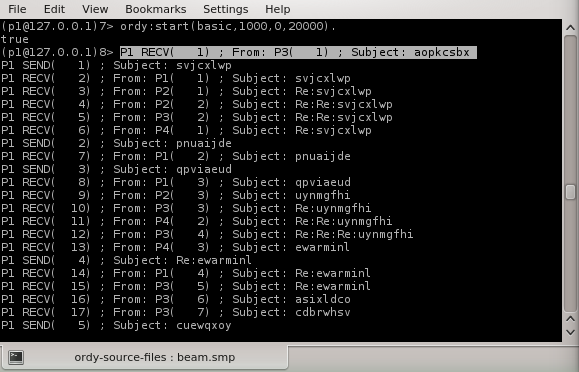
\includegraphics[scale=0.8]{sections/screenshots/p1_basic_jitter0.png}
\caption{P1 - Basic - No Jitter}
\label{fig:p1_basic_no_jitter}
\end{figure}

\begin{figure}[h!]
\centering
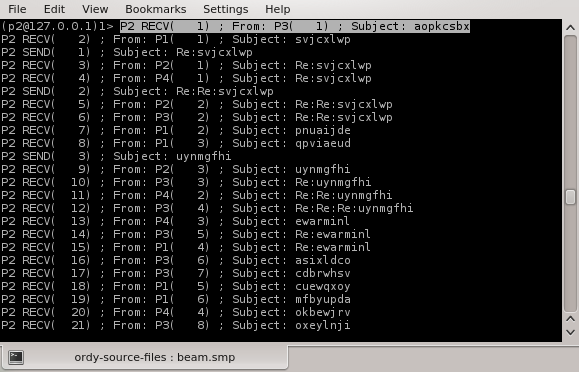
\includegraphics[scale=0.8]{sections/screenshots/p2_basic_jitter0.png}
\caption{P2 - Basic - No Jitter}
\label{fig:p2_basic_no_jitter}
\end{figure}

\begin{figure}[h!]
\centering
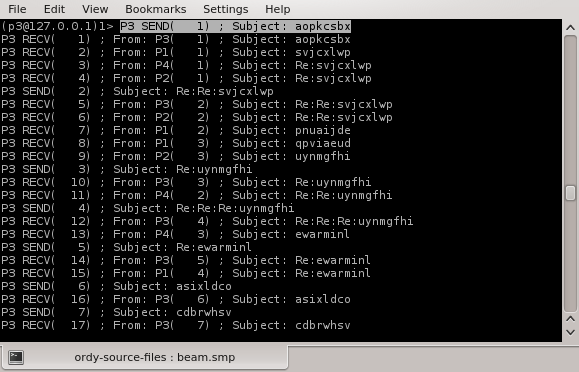
\includegraphics[scale=0.8]{sections/screenshots/p3_basic_jitter0.png}
\caption{P3 - Basic - No Jitter}
\label{fig:p3_basic_no_jitter}
\end{figure}

\begin{figure}[h!]
\centering
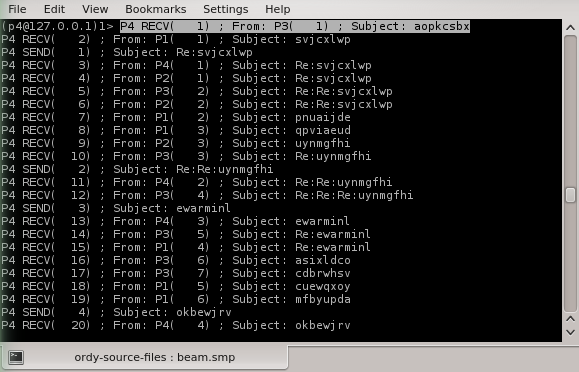
\includegraphics[scale=0.8]{sections/screenshots/p4_basic_jitter0.png}
\caption{P4 - Basic - No Jitter}
\label{fig:p4_basic_no_jitter}
\end{figure}

\clearpage
The second experiment we tried, was to introduce some jitter. You can see there is no causal order, in Figure 6 the higlighted line shows that P2 receives the second answer to a posting before the original posting and the first answer. In the same figure you see that P2 receives the second message that P4 sends before the first. So there is  no FIFO nor causal nor total order, either.


\begin{figure}[h!]
\centering
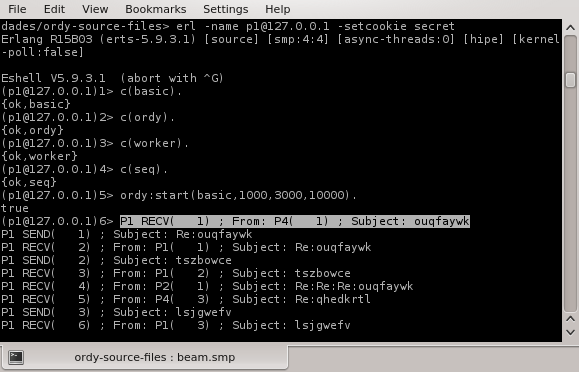
\includegraphics[scale=0.8]{sections/screenshots/p1_basic.png}
\caption{P1 - Basic - Jitter}
\label{fig:p1_basic_jitter}
\end{figure}

\begin{figure}[h!]
\centering
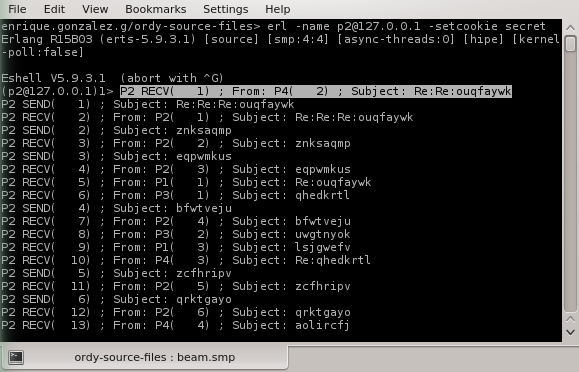
\includegraphics[scale=0.8]{sections/screenshots/p2_basic.png}
\caption{P2 - Basic - Jitter}
\label{fig:p2_basic_jitter}
\end{figure}

\begin{figure}[h!]
\centering
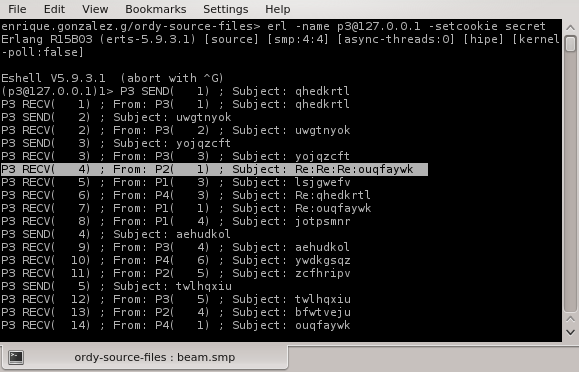
\includegraphics[scale=0.8]{sections/screenshots/p3_basic.png}
\caption{P3 - Basic - Jitter}
\label{fig:p3_basic_jitter}
\end{figure}

\begin{figure}[h!]
\centering
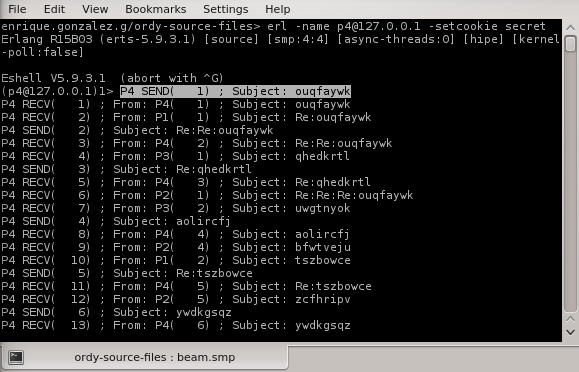
\includegraphics[scale=0.8]{sections/screenshots/p4_basic.png}
\caption{P4 - Basic - Jitter}
\label{fig:p4_basic_jitter}
\end{figure}


\clearpage
\subsection{Causal order multicast}

In this experiment we used the same values as with the experiment with the basic module and jitter. Causal order means that when a process receives a message that it, at least, has all the messages that the sending process had at the moment of sending the message. 
If we take for example the moment at which P1 sends message number 76 than we see that the last message process P1 received from P2 is the message number 66, from P3 number 74 and from P4 number 84. We now just have to look at the output of the other processes and check if at the moment of receiving message number 76 they already have message 66 from P2, 74 from P3 and 84 from P4.
As we can see, we have causal order. Of cause to make sure, that there is casual order, we could have to check the other messages too but it would make this example less clear. In the laboratory we checked that, also with different values.

\begin{figure}[h!]
\centering
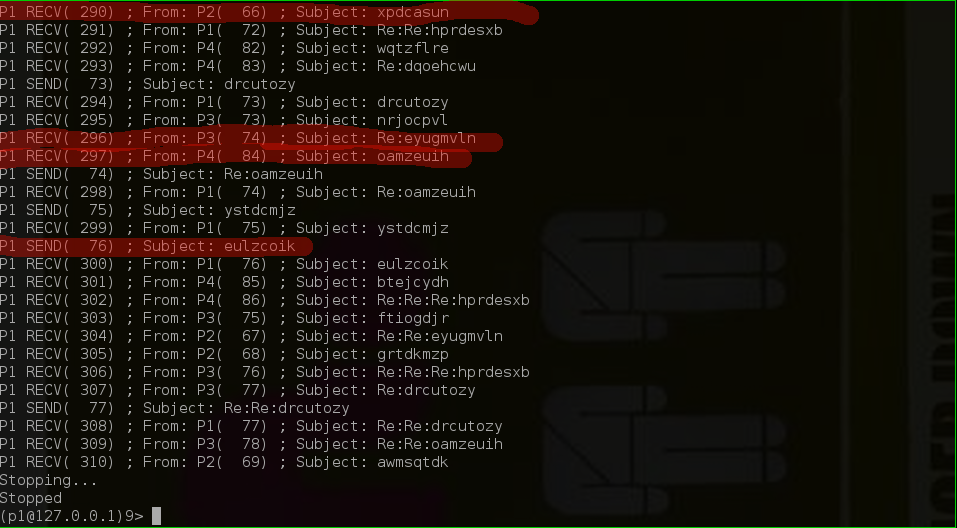
\includegraphics[scale=0.4]{sections/screenshots/causal_p1.png}
\caption{P1 - Causal - Jitter}
\label{fig:p1_causal_jitter}
\end{figure}

\begin{figure}[h!]
\centering
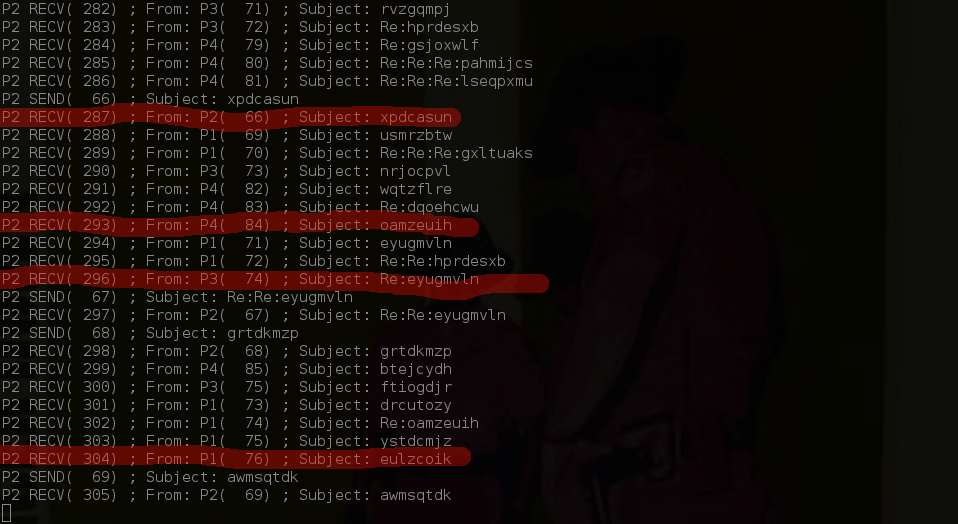
\includegraphics[scale=0.4]{sections/screenshots/causal_p2.png}
\caption{P2 - Causal - Jitter}
\label{fig:p2_causal_jitter}
\end{figure}

\begin{figure}[h!]
\centering
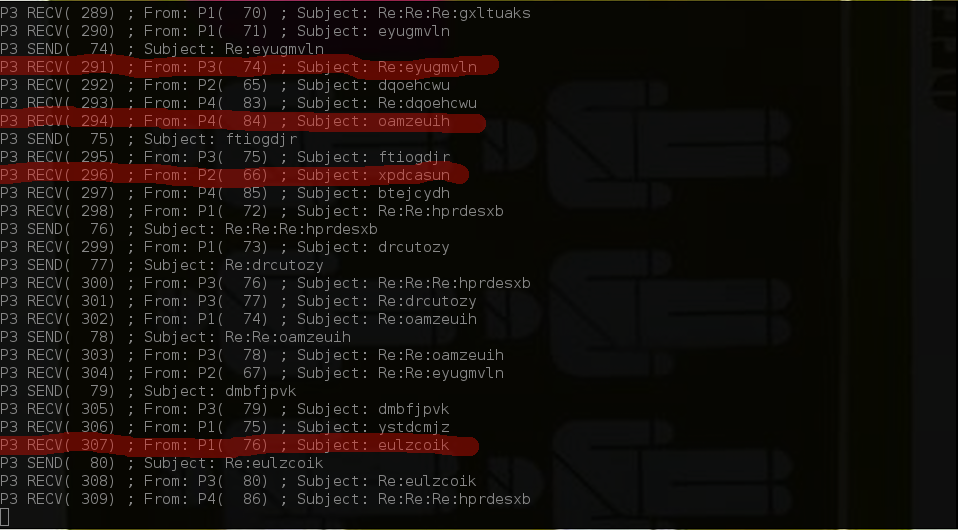
\includegraphics[scale=0.4]{sections/screenshots/causal_p3.png}
\caption{P3 - Causal - Jitter}
\label{fig:p3_causal_jitter}
\end{figure}

\begin{figure}[h!]
\centering
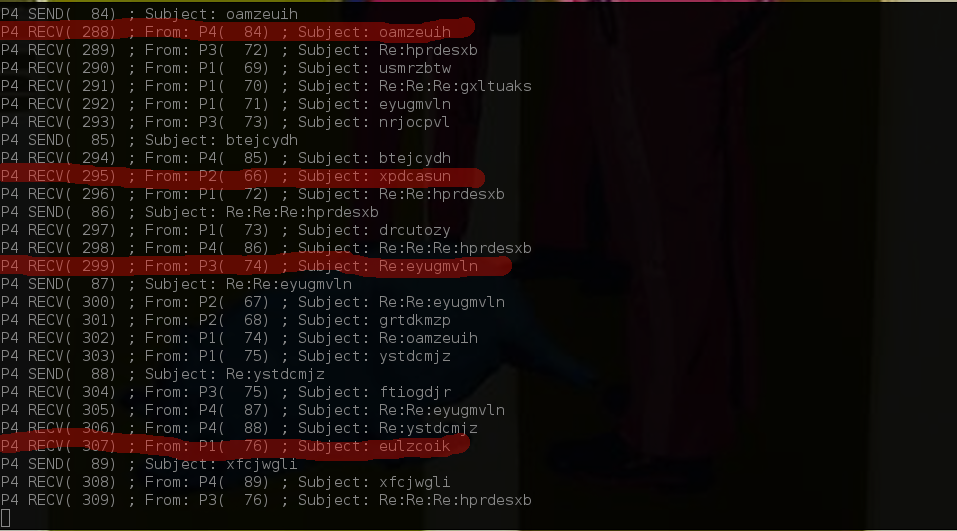
\includegraphics[scale=0.4]{sections/screenshots/causal_p4.png}
\caption{P4 - Causal - Jitter}
\label{fig:p4_causal_jitter}
\end{figure}

\clearpage
\subsection{Total order multicast}
\textit{As we can appreciate in the following screenshots, corresponding to the execution of the program with total order of the posts, the RECV tags appear at the same order in all the figures. The result is always the same, independently the value of jitter. So we can conclude, that we have total order.}

\begin{figure}[h!]
\centering
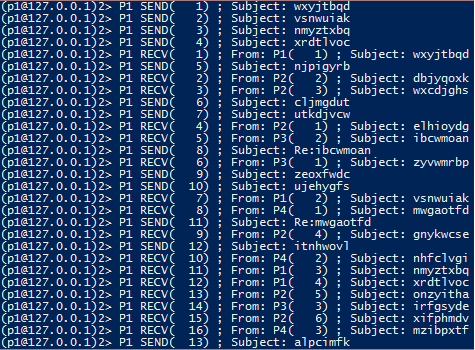
\includegraphics[scale=0.9]{sections/screenshots/totalP1.png}
\caption{P1 - Total}
\label{fig:p1_Total}
\end{figure}

\begin{figure}[h!]
\centering
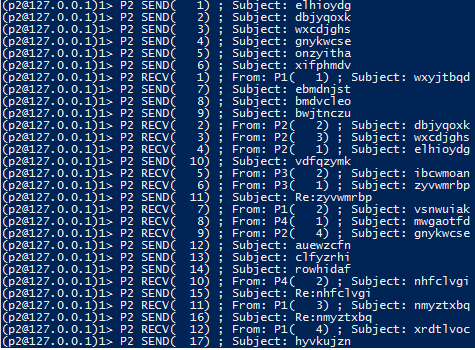
\includegraphics[scale=0.9]{sections/screenshots/totalP2.png}
\caption{P2 - Total}
\label{fig:p2_Total}
\end{figure}

\begin{figure}[h!]
\centering
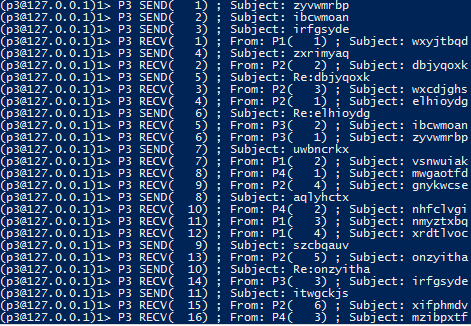
\includegraphics[scale=0.9]{sections/screenshots/totalP3.png}
\caption{P3 - Total}
\label{fig:p3_Total}
\end{figure}

\begin{figure}[h!]
\centering
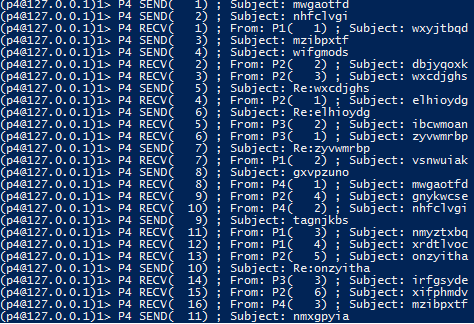
\includegraphics[scale=0.9]{sections/screenshots/totalP4.png}
\caption{P4 - Total}
\label{fig:p4_Total}
\end{figure}

\clearpage
\textit{In this second experiment, we execute our code with the Jitter value equals to 0. In the following Figures, we can appreciate that de order of the RECV tags of each process is the same in all four processes.}

\begin{figure}[h!]
\centering
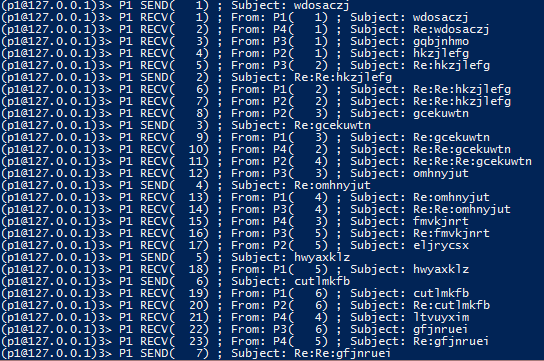
\includegraphics[scale=0.9]{sections/screenshots/totalP1_noJitter.PNG}
\caption{P1 - Total No Jitter}
\label{fig:p1_Total_noJitter}
\end{figure}

\begin{figure}[h!]
\centering
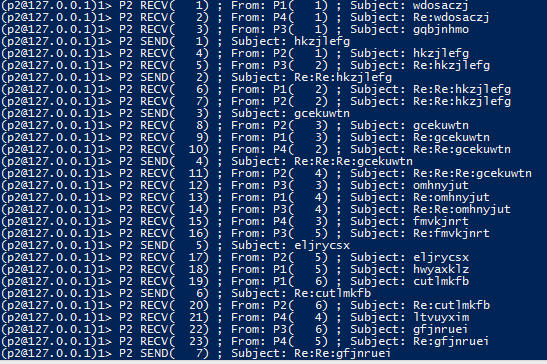
\includegraphics[scale=0.9]{sections/screenshots/totalP2_noJitter.PNG}
\caption{P2 - Total No Jitter}
\label{fig:p2_Total_noJitter}
\end{figure}

\begin{figure}[h!]
\centering
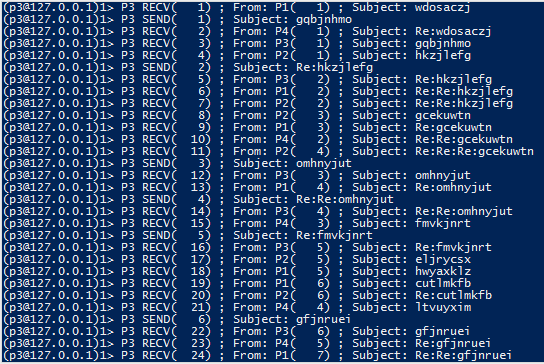
\includegraphics[scale=0.9]{sections/screenshots/totalP3_noJitter.PNG}
\caption{P3 - Total No Jitter}
\label{fig:p3_Total_noJitter}
\end{figure}

\begin{figure}[h!]
\centering
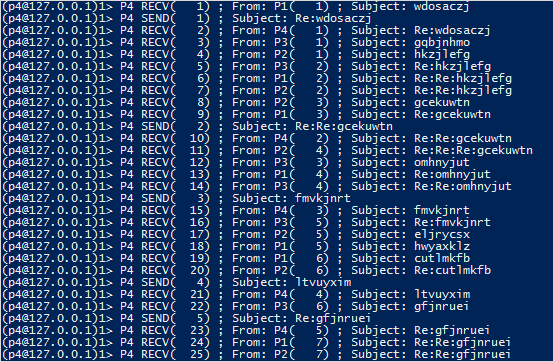
\includegraphics[scale=0.9]{sections/screenshots/totalP4_noJitter.PNG}
\caption{P4 - Total No Jitter}
\label{fig:p4_Total_noJitter}
\end{figure}

\clearpage
\textit{Finally, after many executions in both scenarios (Jitter different to 0 and Jitter equals to 0), we can ansure that the condition of the total order has been satisfied. So we can assume that  the handling of the messages is working properly}